\cleardoublepage

\chapter{Arquitectura e Implementación}
\label{makereference4}

\section{Equipamiento}
\label{makereference4.1}

Existen múltiples niveles de implementación del prototipo planteado en este documento. En función de la cantidad de módulos operativos se requerirá una mayor cantidad de hardware para la sensorización y los actuadores implicados. El nivel más básico e imprescindible implica un ordenador con SO Linux que actuará como controlador de la infraestructura de dispositivos que dan forma al sistema en su conjunto, esto será referido en adelante como el nodo principal.

\section{Definición del nodo principal}
\label{makereference4.2}

El nodo principal representa el núcleo de una suite domótica. Los sensores y actuadores dispuestos en un hogar lo usan como centro neurálgico para que el sistema opere, y la aplicación móvil lo usa como servidor para obtener la información registrada por esos dispositivos e interactuar con ellos. Si bien los sensores son capaces de registrar datos por su cuenta, estos deben ser entregados en el \gls{gateway} para ser procesados de forma útil respeto al resto de la infraestructura. 

\vspace{1cm}

Como soporte de hardware, se usará un ordenador compacto de la marca Raspberry Pi. La selección particular de este dispositivo se apoya en dos características esenciales en el desarrollo de este proyecto: es barato, de bajo consumo eléctrico y aunque no está clasificado como \verb|Open Hardware| ya que la Raspberry Pi Foundation requiere de los ingresos de las ventas de sus distintos modelos de Raspberry, su proyecto goza de buena reputación en el mundo educativo y se considera una organización benéfica con el objetivo de acercar la electrónica a todo el mundo. Además, goza de una gran presencia en el mercado de electrónica, por lo cual es fácil de adquirir y ha acumulado una extensa comunidad de usuarios que muestran su uso mediante tutoriales y experimentos. Como motivos adicionales se encuentra su reducido tamaño que permite ubicarlo con facilidad en lugares estrechos o difícilmente accesibles, además de su imperceptible ruido al operar. El modelo concreto para el desarrollo del prototipo es Rapsberry Pi3b+ que dispone de capacidad de procesador y memoria RAM suficiente para operar todo el software necesario. Este modelo no integra un almacenamiento interno para el usuario, pero su interfaz incluye una ranura de tarjetas micro-SD compatible con prácticamente todas las opciones de tamaño de almacenamiento disponibles en el mercado. Se precisan de al menos 4 \gls{gb} de espacio disponible en la memoria del sistema, y es recomendable exceder este mínimo siempre que sea posible, ya que la acumulación de datos con el paso del tiempo por parte del dispositivo puede crecer indefinidamente.

\vspace{1cm}

El nodo principal ejecuta Raspbian. Un \gls{so} \verb|GNU/Linux| diseñado específicamente para la arquitectura ARMv7 de los distintos modelos de ordenadores Raspberry. Concretamente, en este proyecto se utiliza la serie de distribuciones \verb|Lite|, orientadas a la ejecución del sistema operativa mediante interfaz de linea de comandos en terminal. Esta decisión está fundamentada en desprenderse de la necesidad de periféricos externos e interfaces de \verb|I/O| analógicas para controlar el \gls{so}. Toda configuración del sistema será realizada mediante conexiones por \gls{ssh}. El proceso de instalación y configuración de conexiones esta ampliado en el apéndice~\ref{AppendiA:Key2} del documento.

\vspace{1cm}

Una vez establecidos los medios de comunicación, se instalarán aplicaciones que permitirán ejecutar los servicios necesarios para actuar como nodo central. La estrategia de comunicación entre los distintos dispositivos que conforman la suite domótica se basa en un servidor \verb|NodeJs| que establece conexiones vía \gls{wifi} con los sensores y actuadores mediante el protocolo \gls{mqtt}, y este a su vez con la aplicación móvil vía \gls{wifi} o internet, mediante el protocolo \gls{https}. Se realizara una descripción mas concisa del software necesario en el nodo principal en el apartado \ref{makereference4.3}.



\begin{figure}[hbt!]
\centering
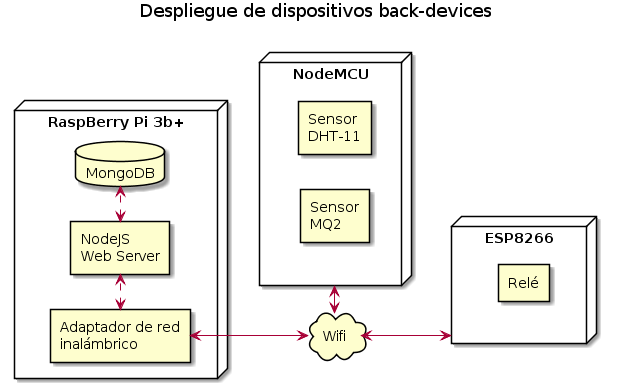
\includegraphics[height=2.5in]{figures/diagrams/physical-devices/back-devices.png}
\caption[Diagrama de despliegue de back-end]{Diagrama de despliegue de dispositivos y gateway\footnotemark}
\end{figure}

\section{Criterio de selección de dispositivos y Software}
\label{makereference4.3}

\begin{figure}[hbt!]
\centering
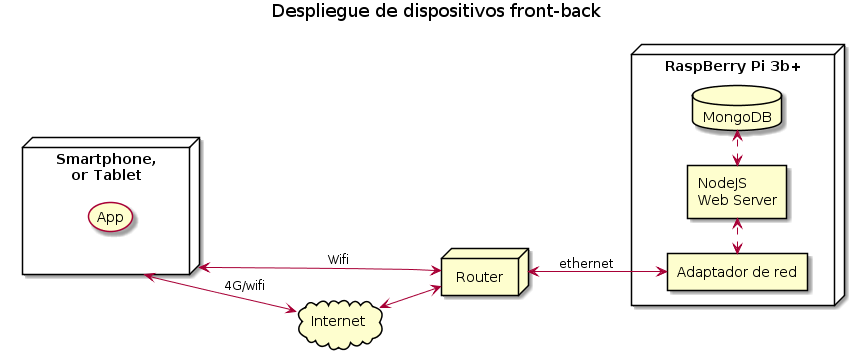
\includegraphics[height=2.5in]{figures/diagrams/physical-devices/front-back.png}
\caption[Despligue de front]{Diagrama de despliegue de smartphone, router y gateway\footnotemark}
\end{figure}

\section{Criterio de selección servicios}
\label{makereference4.4}
La selección de un servicio para la gestión de la \gls{bbdd}


Podría parecer que hablamos de una relación de objetos entre sí, y que un modelo de \gls{bbdd} relacional es la mejor opción, pero si consideramos que, cada entrada almacenada tendrá una estructura distinta, hace que no sea una opción tan ideal. Pensemos, por ejemplo, que utilizando una \gls{bbdd} SQL se planifica un conjunto de tablas relacionadas entre sí. Sera necesaria una tabla que contenga las ubicaciones y se relacione con otra tabla que definan a los dispositivos. Esto establece una relación 1:N donde múltiples dispositivos pueden existir para una estancia, pero nunca en varias a la vez. De cada dispositivo existirá una nueva relación 1:N de medidas. Lo cual deja un esquema semejante al de la figura siguiente:


\begin{figure}[hbt!]
\centering
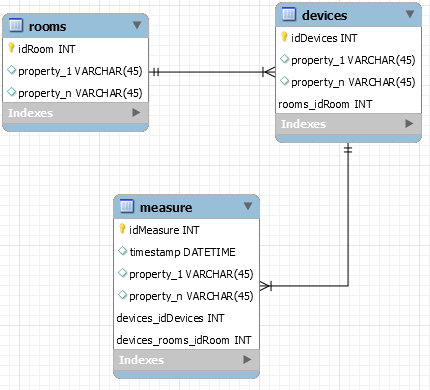
\includegraphics[height=2.5in]{figures/SQLSchemaExample_1.png}
\caption[Primer planteamiento de diseño de BBDD relacional]{Primer planteamiento de diseño de BBDD relacional\footnotemark}
\end{figure}

\vspace{1.5cm}

Sin embargo, existen algunos problemas graves de diseño de esta idea, en primer lugar, los dispositivos no pueden ser una propiedad de una estancia. Son objetos relacionados, pero no existe una transitividad dura entre ellos. Un dispositivo puede cambiar de estancia en un momento dado, y aun asi, seguir existiendo medidas en fechas concretas de ese dispositivo para una habitación en la cual, dicho dispositivo ya no está relacionado. Otro posible escenario es la desaparición de una estancia (como resultado de fusionar 2 estancias en una al derribar una pared). Para mantener una integridad lógica y persistente a lo largo del tiempo. Toda medida deberá tener un campo que determine en que ubicación fue tomada.
no hay transitividad dura entre room y device, lo cual hace que sean independientes entre sí.


\begin{figure}[hbt!]
\centering
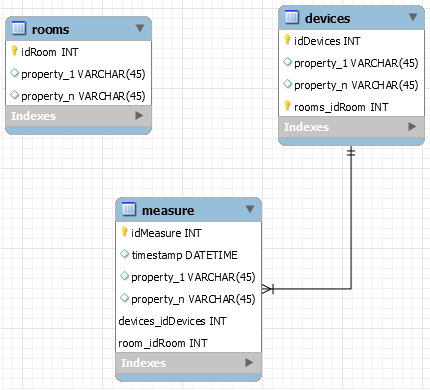
\includegraphics[height=2.5in]{figures/SQLSchemaExample_2.png}
\caption[Segundo planteamiento de diseño de BBDD relacional]{Primer planteamiento de diseño de BBDD relacional\footnotemark}
\end{figure}

\vspace{1.5cm}

Con esto aún tendríamos que enfrentar un problema adicional, el número de columnas que definen las propiedades de una tabla. El ejemplo más claro es la tabla de medidas. Una medida, efectuada por un sensor será definida por su identificador y la fecha en la que se realizó, ahora bien, según la naturaleza del dispositivo, se obtendrán disantos tiempos de medida. Un sensor combinado de temperatura y humedad nos dará dos magnitudes de medición, un sensor de ruido almacenará un valor de decibelios, una luz define su medida por su estado de actividad (encendido o apagado), aunque por otra parte podría indicar el consumo eléctrico, o propiedades adicionales como intensidad de luz, o incluso color. Es cierto que, para un actuador, como lo es un emisor de luz, no realiza medidas como tal, y sus correspondientes estados de actividad podrían ser más adecuados definirlos como propiedades del dispositivo y no como medidas. Podríamos separar las medidas de los estados en tablas distintas, pero igualmente llegaríamos al problema del número de campos necesarios en una tabla. Valor que por otra parte es muy difícil de prever en base a la extensa gama de dispositivos existentes. Esto puede solucionarse de manera sencilla con 2 estrategias. Incluir una gran cantidad de columnas en previsión de los distritos tipos de medidas existentes, dejando que las medidas posean un valor nulo para los campos no utilizados en función de la relación de su sensor, o bien, unificar todos los campos en un único valor de cadena de caracteres que almacene un dato estructurado, como es el caso de los JSON. Esta última opción, sería la más deseable tanto por sencillez de implementación como facilidad de procesamiento. Lo que dejaría un esquema semejante a este:

\begin{figure}[hbt!]
\centering
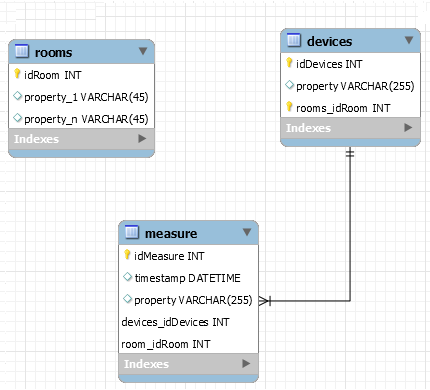
\includegraphics[height=2.5in]{figures/SQLSchemaExample_3.png}
\caption[Tercer planteamiento de diseño de BBDD relacional]{Primer planteamiento de diseño de BBDD relacional\footnotemark}
\end{figure}

Una preocupación que agrava la perspectiva de usar una \gls{bbdd} relacional es, en este punto del proyecto, su escalabilidad horizontal. Si bien las tablas pueden crecer a un gran número de registros, no se prevé almacenar datos con vistas a largo plazo, la mayoría de los valores almacenados serán efímeros en tiempo de utilidad, almacenarlos responde solo a la necesidad de obtener comparativas en plazos de tiempo relativamente cortos, como horas, días, y posiblemente semanas. Mas allá de este rango estos datos no tienen una utilidad real y pueden ser condensados en medias para utilizarse en resúmenes. Por otro lado, disponer de flexibilidad a la hora de configurar la extensión de propiedades de un objeto de la \gls{bbdd} es uno de los puntos fuertes de una \gls{bbdd} no relacional.


\section{Arquitectura de la aplicación frontend}
\label{makereference4.5}

\subsection{Consideraciones previas}
\label{makereference4.5.1}

El desarrollo de la app frontend se ha servido de dos frameworks para salvar ciertos escollos básicos no relacionados con la implementación de la suite domótica. Por un lado, se ha hecho uso del framework Open Source Ionic (en su versión 3), que es un framework Open Source para la construcción de aplicaciones híbridas multiplataforma, que nos permitirá portar la aplicación para cualquier dispositivo móvil Android a través de Cordova, y que además nos permitirá hacer uso de capacidades nativas de los dispositivos móviles (como el módulo de Wifi) gracias a los plugins existentes para ello. Además, Ionic proporciona grandes herramientas en cuanto a la maquetación responsive, lo cual ayuda en la creación de una aplicación móvil sin necesidad de invertir grandes esfuerzos en alcanzar un aspecto, usabilidad y elegancia mínimos y pudiendo redirigir ese esfuerzo a otros terrenos más fructíferos. Ionic está basado en Angular, el otro framework del que se ha hecho uso (en su versión 5) especialmente por su enfoque en una arquitectura basada en componentes que puedan ser reutilizados con mucha facilidad a lo largo de toda la aplicación. Las versiones modernas de Angular hacen uso de TypeScript para la programación de su lógica de negocio, lo que permite una mayor limpieza de código, mejores herramientas de tipado estricto y redunda en mayor escalabilidad. Angular se programa en TypeScript para la lógica de negocio, SASS para los estilos css y HTML para la maquetación.

\vspace{0.5cm}

\subsection{Estructura básica}
\label{makereference4.5.2}

A grandes rasgos, la aplicación frontend está estructurada en:
\begin{enumerate}
 \item Componentes, por lo general tendremos casi tantos como trozos o segmentos en los que se quiera desestructurar una vista (los conoceremos como \textit{component}; serán útiles para aislar los diferentes comportamientos que se puede requerir en cada vista, y un mismo componente puede ser replicado infinitamente a lo largo de la aplicación cada vez con unos parámetros diferentes.
 \item Módulos de vistas, generalmente uno por cada vista de la aplicación (lo que conoceremos como \textit{view} o \textit{template}); se encargarán de cargar la información que requiere la vista y de transformar las interacciones del usuario con la vista en flujos lógicos que generalmente pasan por (o acaban en) otros módulos.
 \item Centros de gestión y manipulación de datos, generalmente uno por cada estructura de datos existente (lo que conoceremos como \textit{store}); su cometido será proporcionar métodos a otros módulos o vistas para obtención y/o manipulación de su tipo de datos, siendo la store la responsable última de obtenerlos, manipularlos o almacenarlos por cualquier medio existente.
 \item Servicios que ejercerán de cómodas APIs contra APIs externas o contra \gls{bbdd} locales del dispositivo (los que conoceremos como \textit{api provider/service} en el primer caso y \textit{database service} en el segundo), generalmente uno de cada por cada estructura de datos existente; son responsables de lanzar las llamadas a dichos servicios con los parámetros adecuados (bien seas APIs REST remotas o \gls{bbdd} locales) y controlar sus respuestas.
 \item Servicios, que implementan utilidades y herramientas a lo largo de toda la aplicación de forma independiente, tanto que, técnicamente, podrían formar parte de cualquier otra aplicación (los que conoceremos como \textit{service}); son responsables de aportar utilidades puntuales con la suficiente abstracción como para que el "usuario" de dicho servicio no conozca su funcionamiento en detalle, sino más bien, le resulte sencillo, conveniente y cómodo acudir a sus métodos.
\end{enumerate}

\vspace{0.5cm}

Con el fin de comprender el esquema utilizado, mencionaremos los tipos de estructura existentes, aun cuando detallaremos su flujo más adelante: tendremos los dispositivos, que serán conocidos como \textit{things} (siendo posiblemente lo más adecuado debido a su famosa acepción en el \gls{iot}); las habitaciones, que mencionaremos aquí y allá como \textit{rooms}; los usuarios, que conoceremos como \textit{users}; las placas, que mencionaremos como \textit{boards}; y los datos de aplicación generales, a los que nos referiremos como \textit{application data}. Se observará que, en todos los casos, nos conviene referirlos en su traducción al inglés por facilidad a la hora de seguir el hilo del flujo en el código.

\subsection{Patrón del flujo de datos}
\label{makereference4.5.3}

En pro de aplicar una arquitectura que intenta aplicar los principios de separación de responsabilidades y capas de abstracción, a continuación explicamos los patrones que sigue la estructura del proyecto frontend.

\begin{figure}[hbt!]
\centering
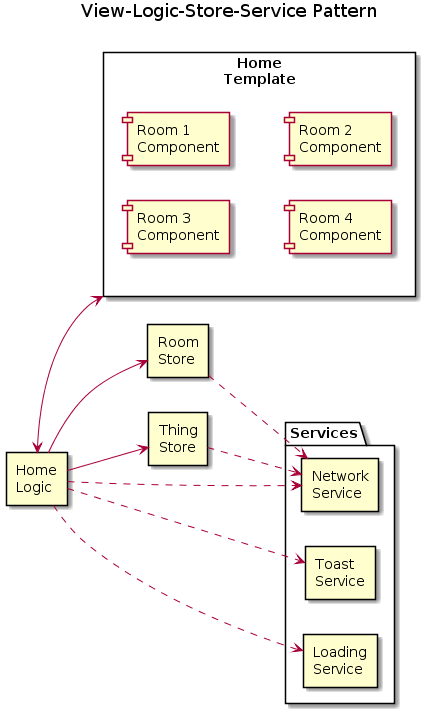
\includegraphics[height=5in]{figures/diagrams/front/architecture/view-logic-store-service-pattern.png}
\caption[view-logic-store-service-pattern]{View-Logic-Store-Service Pattern\footnotemark}
\label{fig:front-view-store}
\end{figure}

\vspace{0.5cm}

Por lo general, todas las vistas presentan, bajo un formato u otro, una serie de datos. El template será por tanto responsable de adaptar y mostrar estos datos como se requiera; pero primero deben obtenerlos, para lo cual delegarán en la store. A partir del momento en que se pide estos datos a la store, se crea una conveniente capa de abstracción que es útil en dos sentidos principales: por un lado, la vista no debe preocuparse del origen de dónde obtener esos datos, esto será responsabilidad de la store, lo cual hace más limpio el código del template, que debe preocuparse estrictamente de atender a los requisitos y cambios de la vista; por otro, la misma lógica que deba implementar la store para ofrecer estos datos a una vista, podrá ser reaprovechada para ofrecérselo a otra. 

\vspace{0.5cm}

En el ejemplo de la Figura \ref{fig:front-view-store}, podemos observar como el template de la vista \textit{Home} debe mostrar una lista de todas las habitaciones existentes. Una vez el template ha adquirido este array de rooms a partir de la room store, deberemos mostrar un componente room por cada room en esa lista. Sin embargo, la longitud de esta lista no es conocida de antemano, y puede cambiar en cualquier momento. Por tanto, la implementación debe ajustarse a este dinamismo. Angular nos permite, mediante su directiva \textit{ngFor}, generar tantos elementos como existan en un array de la lógica asociada al template, y además pueden ser elementos de cualquier tipo, luego esto nos sirve para crear una lista de componentes room, siendo posible instanciar cada uno con la información específica de cada elemento del array.

\vspace{0.5cm}

Observaremos que tanto la lógica asociada a una vista como las stores (así como otros services) hacen uso de los services. Estos services ofrecen, de forma autónoma e independiente, ciertas utilidades, como por ejemplo el LoadingService, que ofrece un spinner de carga con un mensaje de feedback para el usuario de que un proceso está cargando. El encargado de poseer y ejecutar la lógica que crea y muestra el spinner será el LoadingService; sin embargo, quien manda la orden inicial será siempre quien invoca al servicio, pues es quien conoce el estado actual de la vista: si los datos han sido pedidos y está a la espera de recibirlos, pedirá mostrar el spinner; si finalmente se recibe confirmación de que la vista ya tiene disponibles los datos, se ordenará ocultar el spinner. 

\vspace{1cm}

\begin{figure}[hbt!]
\centering
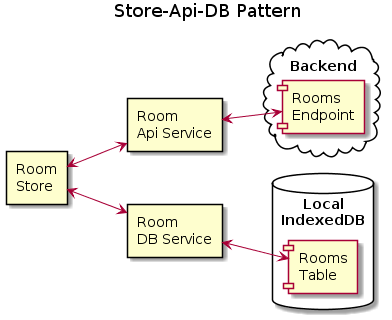
\includegraphics[height=2.5in]{figures/diagrams/front/architecture/store-api-db-pattern.png}
\caption[store-api-db-pattern]{Store-API-DB Pattern\footnotemark}
\label{fig:front-store-api-db}
\end{figure}

Respecto a la obtención de los datos, utilizamos el patrón asociado a la Figura \ref{fig:front-store-api-db}. La store mantiene el rol más importante del flujo del frontend. Observaremos que, cada vez que un componente, vista o módulo desea interactuar con un ejemplar del tipo que regenta la store, por ejemplo, cada vez que un módulo desee obtener la información de una determinada habitación o desee cambiar uno de sus parámetros, pedirá esa información o ese cambio a la room store. Será en ese momento cuando la store decidirá de dónde obtener la información del objeto room, o a qué servicio externo (API o \gls{bbdd} local) hacerle la petición de cambio. Así, veremos que la store hará las veces de distribuidor de la información de su tipo.

\vspace{0.5cm}

En este punto, con el fin de ejercer la separación de responsabilidades, hemos creado un módulo api provider (específicamente orientado para el mismo tipo de datos que la store) que permite a la store interactuar con la api remota de su mismo tipo; así, cuando la room store quiere obtener del backend la última lista real de rooms disponibles, hará uso del método \verb|getAllRooms| del room provider; de la misma forma, cuando bajo petición del usuario, quiera crear una nueva room, debe hacerse esta petición al servidor a través del método \verb|createRoom| del room provider. Cada una de estas peticiones http a la API remota puede requerir de unas características particulares, como puedan ser su tipo CRUD, los headers http requeridos, la url particular de la petición y la estructura del cuerpo; y al delegar en el api provider, se evitar exponer a la store detalles intrínsecos a la petición http, que debería resultar comportarse como una caja negra de cara a la store, ya que no requiere ese nivel de detalle para su cometido de distribuir la información. 
Es necesario apuntar que todos los api service que hemos creado (en general un por cada tipo de dato importante, o quizás más precisamente, uno por cada endpoint de entrada existente en la API remota), heredan de la clase ApiGenericProvider, la que implementa los métodos CRUD con los que interactuar con la API remota. En la Figura \ref{fig:api-services} se expone el diagrama de clases para todas las APIs creadas.

\begin{figure}[hbt!]
\centering
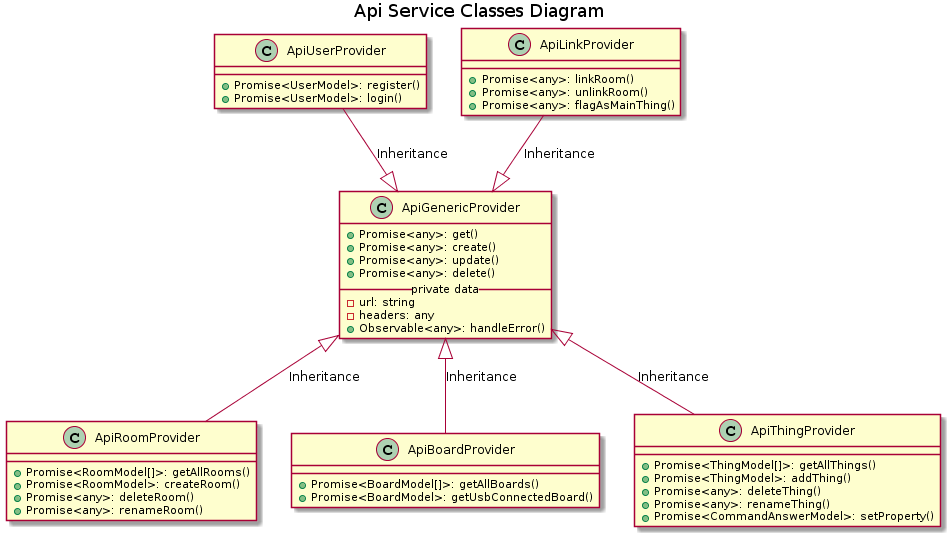
\includegraphics[height=4in]{figures/diagrams/front/architecture/api-services.png}
\caption[api-services]{API Providers Class Diagram\footnotemark}
\label{fig:api-services}
\end{figure}

\vspace{0.5cm}

De la misma forma y con el mismo objetivo que para el api provider, se crea un módulo database service (específicamente orientado para el mismo tipo de datos que la store), que permite a la store interactuar con la \gls{bbdd} local para almacenar, recuperar o borrar cualquier entrada de ese tipo. En este proyecto, de entre las posibilidades existentes, hacemos uso de la base de datos IndexedDB, propia del motor web del dispositivo. Es una base de datos No-SQL que está orientada al almacenamiento de entradas de gran tamaño, y no bloquea la entrada-salida del hilo principal, de forma que es ideal para almacenar objetos JSON, que puedan tener estructuras y tamaños variables. En particular, cada database service se creará de forma que ataque específicamente a una única tabla, nombrada con el mismo tipo de datos, con el objetivo de reforzar la mantenibilidad del código y la separación de responsabilidades. Así, de nuevo, la store se permite desconocer si sus datos deben tener una estructura, codificación o formato en particular dependiendo de las características de la \gls{bbdd}: delega esa responsabilidad en el database service, el cual debe garantizar que los datos sean devueltos a la store en el mismo formato en que fueron entregados en primera instancia. 
Los módulos database service, a diferencia de los api providers, no heredan de un mismo módulo, pero queda pendiente como una mejora posible puesto que cada uno puede ser creado con una configuración particular (como ya ocurre) y, con la excepción de algunos métodos, se puede refactorizar todos aquellos que sean comunes en una clase padre. En la Figura \ref{fig:database-service} se expone la clase que sigue RoomDatabaseService, muy similar a la que siguen el resto de database services con sus configuraciones propias. Hemos adjuntado un diagrama de cada uno de ellos en el apartado \ref{makereference4.5.4}.


\begin{figure}[hbt!]
\centering
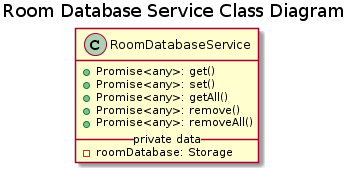
\includegraphics[height=1.5in]{figures/diagrams/front/architecture/database-service.png}
\caption[app-data]{Room Database Service Class Diagram\footnotemark}
\label{fig:database-service}
\end{figure}

\subsection{Diagramas de clases de las Stores, Models y Services}
\label{makereference4.5.4}

[EXPLICAR AQUÍ EL PROCESO DE INICIALIZACIÓN DE LA APP]

\subsection{Diagramas de clases de las Stores, Models y Services}
\label{makereference4.5.5}

\begin{figure}[hbt!]
\centering
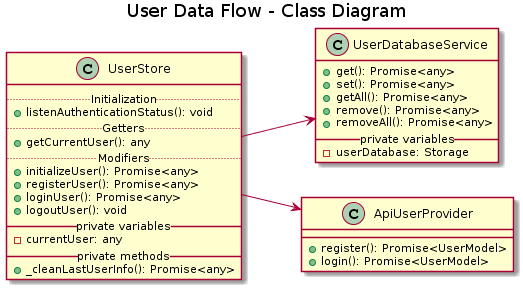
\includegraphics[height=2.5in]{figures/diagrams/front/data-flow/user.png}
\caption[user]{User Data Class Diagram\footnotemark}
\end{figure}

La user store gestiona todo lo relacionado con el login del usuario, es por ello que tiene una fuerte cooperación con el AuthService. Durante la inicialización de la aplicación, se establece una suscripción a cambios de usuarios autenticados en el AuthService con el método público \verb|listenAuthenticationStatus|.

\vspace{0.5cm}

Nuestro proyecto implementa JWT de Auth0, para la autenticación de usuario mediante tokens, lo cual agiliza el login sin necesidad de que el usuario deba introducir de nuevo sus credenciales, y puede ser parametrizado desde el backend. Durante la inicialización de la aplicación, se lanza el método \verb|initializeUser|, el cual busca en la userDB (local del dispositivo) la existencia de un JWT válido. Si lo encuentra, entonces puede pasarle el token al AuthService, el cual lo descifrará y extraerá el usuario autenticado, y establecerá el estado de autenticado del AuthService a verdadero. De esta manera, se la suscripción del \verb|listenAuthenticationStatus| da lugar a pedirle a AuthService el usuario autenticado y se establece como el usuario actual. Si no, se lanza el método privado \verb|_cleanLastUserInfo| para borrar cualquier información remanente en la aplicación móvil relativa al último usuario logado, acudiendo a todas las demás stores para que se encarguen de borrar de sus \gls{bbdd} locales la información pertinente de la que son responsables.

\vspace{0.5cm}

Además de esto, la user store posee los métodos \verb|loginUser| y \verb|registerUser| que gestionan todo lo relacionado con los intentos de registrar y de iniciar sesión contra la API remota de user mediante el userProvider. Si logra logarse correctamente, el endpoint de login devuelve un token válido que la app almacena en la userDB y que utiliza para el propósito explicado anteriormente, además de pasar al AuthService este token válido para autenticar al usuario.

\begin{figure}[hbt!]
\centering
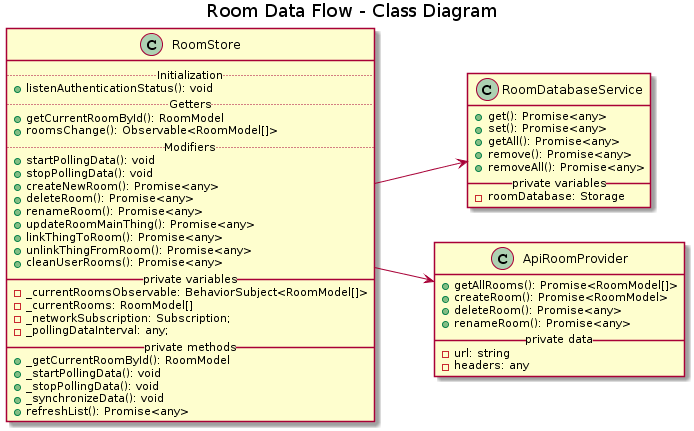
\includegraphics[height=3.5in]{figures/diagrams/front/data-flow/room.png}
\caption[room]{Room Data Class Diagram\footnotemark}
\end{figure}

\vspace{1cm}

La room store gestiona todo lo relacionado con la lista de rooms disponibles. Durante la inicialización de la aplicación, se establece una suscripción a cambios de usuarios autenticados en el AuthService con el método público \verb|listenAuthenticationStatus|; y alinea esta suscripción con otra al estado de la red con el NetworkService, de forma que, si hay conexión a la red y además el usuario está autenticado, se llama al método privado \verb|_startPollingData| (y de lo contrario, llama al \verb|_stopPollingData|).

\vspace{0.5cm}

\verb|_startPollingData| se encarga de llamar a intervalos de tiempo regulares de 5 segundos al método privado \verb|_synchronizeData|, el cual hace uso del roomProvider para obtener la lista de todas las rooms. Cada vez que interactuemos con la API remota (con cualquiera de sus métodos, y aplicable al resto de stores), ejecutaremos un flujo que consiste en recibir la información, guardarla en la roomDB y llamar al método \verb|refreshList|, que se encarga de extraer el valor actual de esa lista de la roomDB y actualizar tanto el array privado \verb|_currentRooms| como el observable \verb|_currentRoomsObservable| con el nuevo valor.

\vspace{0.5cm}

Este último paso es crucial para el flujo de datos en la aplicación y representa uno de los patrones reconocidos más útiles de los que hacemos uso en la aplicación frontend: el patrón Observer/Subscribe. La librería RXJs nos ofrece este elemento tan importante, mediante el cual cualquier flujo de la aplicación que desee hacer uso de la lista de rooms, se suscribe al observable \verb|_currentRoomsObservable| mediante el método \verb|roomsChange| de la room store. Cada vez que la room store actualice este observable, el cambio será automáticamente notificado a todos los suscriptores de dicho observable.

\vspace{0.5cm}

La room store también ofrece los métodos \verb|createNewRoom|, \verb|deleteRoom|, \verb|renameRoom|, \verb|updateRoomMainThing|, \verb|linkThingToRoom| y \verb|unlinkThingFromRoom|. Los tres primeros son autodescriptivos, interactuan con la API y siguen el mismo flujo de actualización descrito anteriormente aunque adaptado a cada caso. Los tres últimos son llamados desde la thing store como parte de unos procesos encadenados, en los cuales se requiere que se cambie información específica de alguna room en particular, pero esta vez sólo de forma local (en el dispositivo), ya que la petición al backend realizada desde la thing store ya desencadena otros flujos secundarios en el backend que actualizan la información de la room implicada. Se garantiza la alineación de datos ya que el flujo está diseñado como si de una transacción se tratara: el backend siempre tiene la información verídica, y si ocurriera algún fallo en el flujo (sea en backend o en frontend), se rechaza el flujo para evitar datos incorrectos, que en cualquier caso serán actualizados con la siguiente petición \verb|_synchronizeData|. 
La room store también expone el método \verb|cleanUserRooms|, accedido y usado desde la user store para el borrado de datos de rooms.

\begin{figure}[hbt!]
\centering
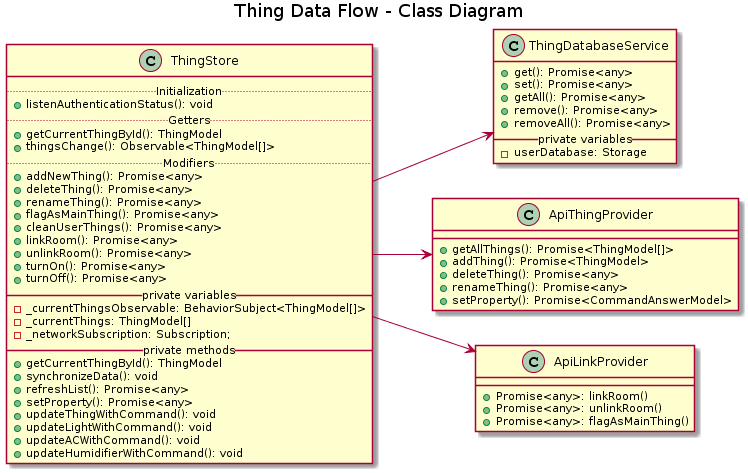
\includegraphics[height=4in]{figures/diagrams/front/data-flow/thing.png}
\caption[thing]{Thing Data Class Diagram\footnotemark}
\end{figure}

La thing store gestiona todo lo relacionado con la lista de things disponibles. Tanto la suscripción al AuthService, y al NetworkService, como el sistema de petición periódica y recuperación de datos, así como la exposición del observable a posibles suscriptores, es idéntico al de room store pero evidentemente aplicado a la lista de things, por lo cual no entraremos en detalle de nuevo.

\vspace{0.5cm}

La thing store también ofrece los métodos \verb|addNewThing|, \verb|deleteThing|, \verb|renameThing|, \verb|flagAsMainThing|, \verb|linkRoom| y \verb|unlinkRoom|, que interactuan con la API en sus métodos homónimos y siguen el mismo flujo de actualización descrito anteriormente aunque adaptado a cada caso. Los tres últimos 

La thing store también expone el método \verb|cleanUserThings|, accedido y usado desde la user store para el borrado de datos de things.


\begin{figure}[hbt!]
\centering
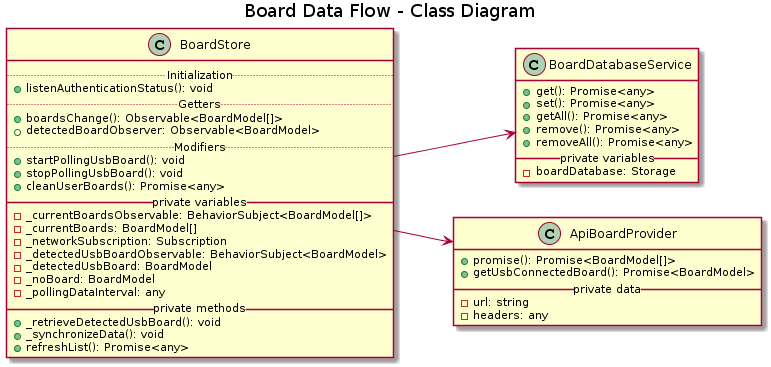
\includegraphics[height=3.5in]{figures/diagrams/front/data-flow/board.png}
\caption[thing]{Board Data Class Diagram\footnotemark}
\end{figure}

[EXPLICAR AQUÍ EL BOARD STORE]

\begin{figure}[hbt!]
\centering
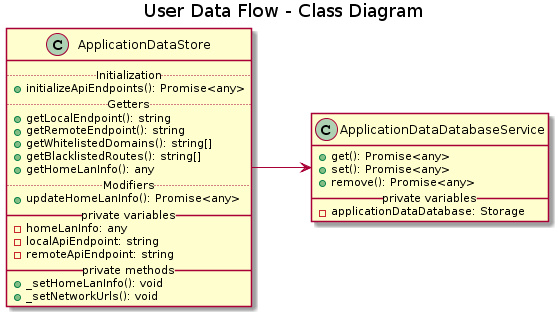
\includegraphics[height=3in]{figures/diagrams/front/data-flow/app-data.png}
\caption[app-data]{Application Data Class Diagram\footnotemark}
\end{figure}

[EXPLICAR AQUÍ EL APP DATA STORE]

\begin{figure}[hbt!]
\centering
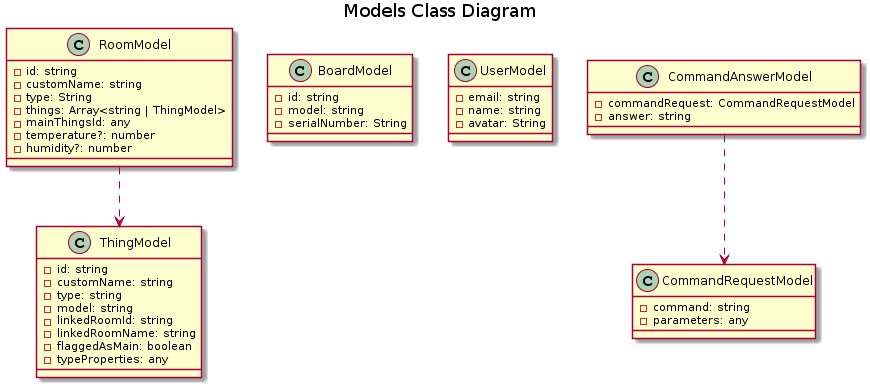
\includegraphics[height=3in]{figures/diagrams/front/architecture/models.png}
\caption[models]{Models Classes Diagram\footnotemark}
\end{figure}

[EXPLICAR AQUÍ LOS MODELS]

\begin{figure}[hbt!]
\centering
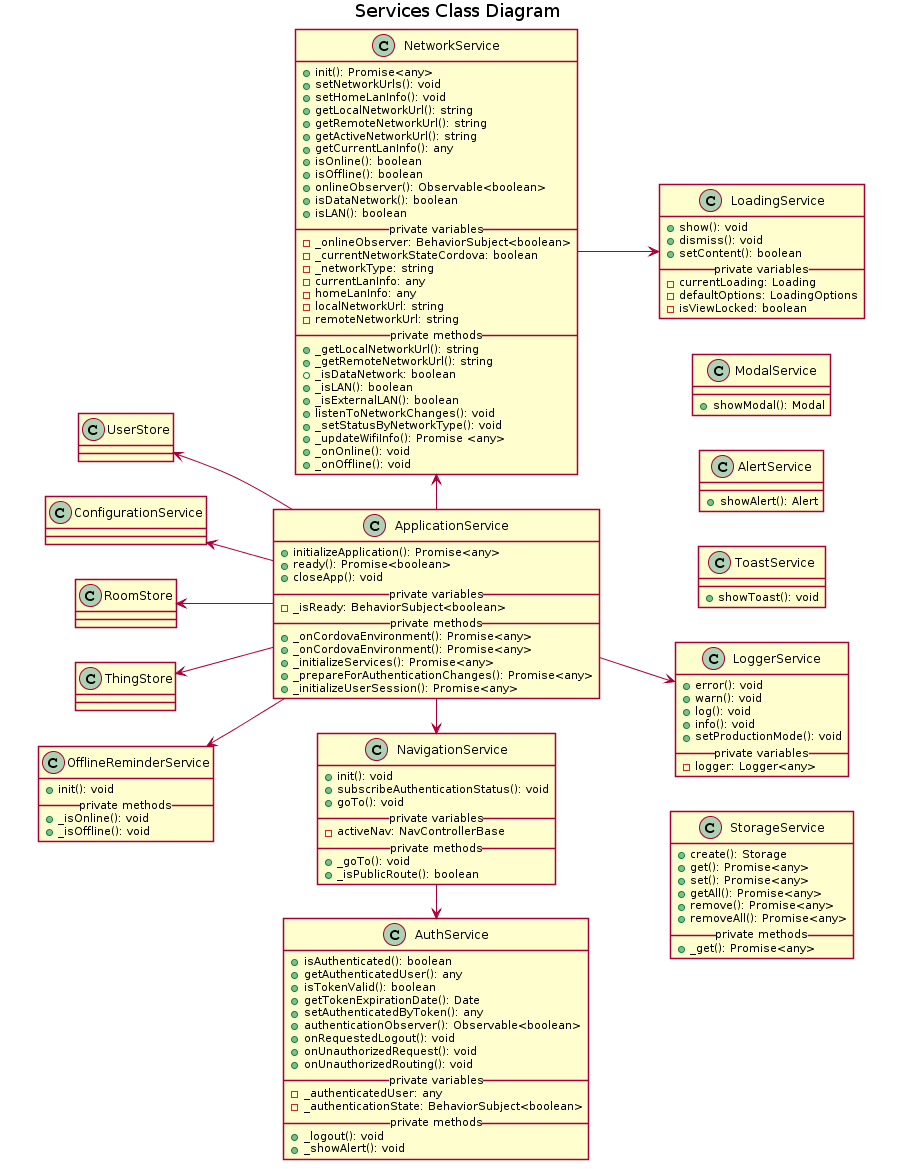
\includegraphics[height=8.5in]{figures/diagrams/front/architecture/services.png}
\caption[services]{Services Class Diagram\footnotemark}
\end{figure}

[EXPLICAR AQUÍ LOS SERVICES]

\section{Arquitectura del servidor de NodeJS}
\label{makereference4.6}

\subsection{Consideraciones previas}
\label{makereference4.6.1}

El desarrollo de la aplicación backend ha seguido la línea del stack MEAN, esto es, MongoDB, ExpressJS, Angular (éste sólo en el frontend) y NodeJS. Los beneficios de seguir dicho stack son sencillamente los de sus frameworks y herramientas: MongoDB aporta los beneficios de una \gls{bbdd} no relacional, enormemente alineado con las características del proyecto, según el cual podríamos almacenar grandes cantidades de datos con diferentes estructuras JSON bajo la misma lista de documentos sin perder velocidad de acceso o escritura; ExpressJS nos permite elaborar una API REST completa salvando los principales escollos que NodeJS podría presentarnos para tal fin, pues sus herramientas base para el tratamiento de peticiones http se presentan intrincadas y poco intuitivas; y NodeJS se beneficia de infinitas librerías de sencillo uso, constantemente probadas y actualizadas por su amplia comunidad, proveyéndonos en este caso de muchas utilidades que nos ayudan a evitar desarrollos difíciles e innecesarios no intrínsecos a una suite domótica (como es nuestro fin) y cuyos beneficios enumeraremos más adelante.

\subsection{Estructura básica}
\label{makereference4.6.2}

A grandes rasgos, la aplicación backend está estructurada en:
\begin{enumerate}
 \item Enrutadores, por lo general tendremos uno por cada nombre en nuestra API REST (los conoceremos como \textit{routers}); gracias a ExpressJS, permiten encaminar cada petición http recibida en el servidor según su tipo CRUD (GET, POST, PUT o DELETE) y la estructura de la URL asociada, para ser atendida por el método específico que debe procesar dicha petición.
 \item Controladores, por lo general tendremos uno por cada nombre en nuestra API REST (los conoceremos como \textit{controllers}); encuadran un contexto en el que se crea, manipula, sirve, guarda y destruye elementos de la estructura de datos asociada, además de exponer una serie de métodos, generalmente uno por cada posible entrada de la API para el nombre de dicha API asociado a la estructura de datos en uso.
 \item Modelos, de los que tendremos uno por cada estructura de datos existente (los conoceremos como \textit{models}); definirán la estructura JSON que debe seguir un objeto para ser incluido en una collección de MongoDB, y que utilizaremos para generar y reconocer objetos de dicho tipo de estructura de datos y poder mejorar la interacción con la \gls{bbdd} de MongoDB.
 \item Servicios, que al igual que en el proyecto frotend, ejercerán de cómodas APIs contra diferentes servicios, como pueda ser la \gls{bbdd} de MongoDB, el protocolo \gls{mqtt} y otros módulos de utilidades (los conoceremos como \textit{providers} o \textit{services}); por lo general, podrían ser prácticamente independientes y ser copiados tal cual a cualquier otro proyecto (a falta de ligeras adaptaciones que en lineas generales facilitan su explotación en cada caso) y proporcionan una capa de abstracción adicional que delimita la responsabilidad del módulo que hace uso de dicho servicio y reduce su complejidad de código.
 \item Módulos de soporte, por lo general tendremos tantos como sean necesarios, y cada uno se dedica exclusivamente a un tipo de estructura de datos (los conoceremos como helpers); ofrecen sus métodos tanto a su controller asociado como a otros controllers, de forma desacoplada con el fin de aligerar la carga de código del controller asociado.
 \item Módulos intermediarios, que aportan utilidades adicionales a la hora de procesar peticiones http (los conoceremos como \textit{middlewares}); gracias a ExpressJS, permitirán enriquecer el tratamiento de dichas peticiones para establecer filtros adicionales o transformaciones de los datos de la petición.
 \item Archivos de configuración y de constantes, que permitirán aislar adecuadamente el uso de constantes útiles a lo largo de toda la aplicación, de una forma centralizada, independiente y de fácil acceso y modificación.
\end{enumerate}

Con el fin de comprender el esquema utilizado y establecer una alineación con el frontend, la nomenclatura utilizada para cada tipo de datos será la misma que en el proyecto cliente.

\subsection{Flujo de enrutado de las peticiones HTTP}
\label{makereference4.6.3}

\begin{figure}[hbt!]
\centering
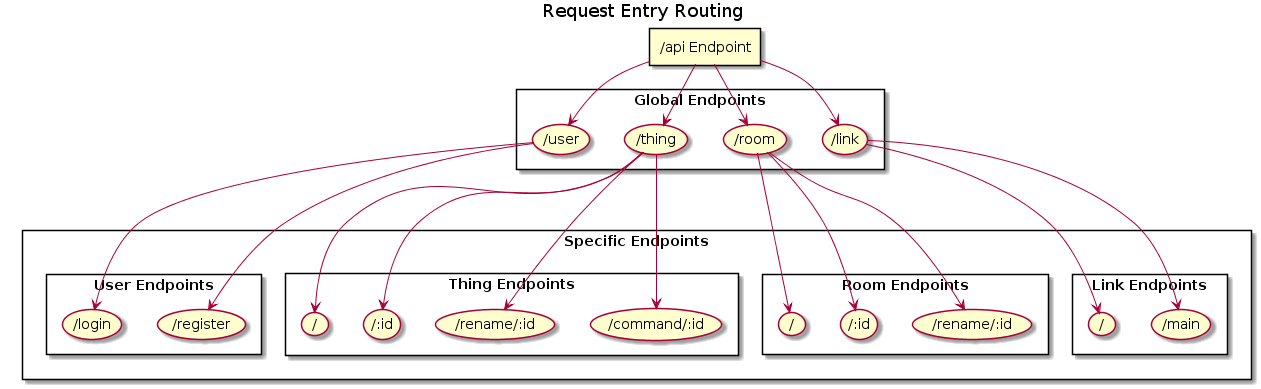
\includegraphics[height=2.5in]{figures/diagrams/back/router-flow/api-entry.png}
\caption[api-entry]{Base API Entry Schema\footnotemark}
\label{fig:back-api-entry}
\end{figure}

Como hemos explicado anteriormente, ExpressJS es utilizado para el enrutado de toda petición HTTP que alcance la aplicación backend. Durante la inicialización del servidor, mediante el método \verb|listen| en el \verb|server.js| se utiliza el objeto \verb|app| expuesto en el \verb|src/app.js| (un objeto generado por el framework ExpressJS) para generar un servidor que atenderá todas las peticiones HTTP en el puerto que se le configure, en este caso, se ha designado el puerto 3000.
\vspace{0.5cm}
Posteriormente, se lanza el setup del enrutador con el método \verb|setupRouting| del módulo \verb|router.js|, el cual se encarga de importar todos los routers existentes y vincularlos a cada uno de los endpoints que serán atendidos mediante el método \verb|use| del objeto \verb|app|. Así, suponiendo que se recibe una petición http con la ruta \verb|/api/thing|, ésta será redirigida al router \verb|thingRouter| mediante el método y sus parámetros \verb|use(ROUTER_CONFIG.EP_GLOBAL.THINGS, thingRouter)|. El primer nivel de encaminamiento de las peticiones es tal que el mostrado en la Figura \ref{fig:back-api-entry}.
\vspace{0.5cm}
Una vez la petición ha sido encaminada a un router en particular, entramos en el segundo nivel de encaminamiento. En este punto, el router se encarga de importar el controller específico para su tipo de datos y de encaminar cada endpoint a la función final de un controller que atenderá a dicha petición. ExpressJS nos permite registrar dicha función a ejecutar para unas características particulares de petición, de forma que con unos sencillos métodos, podremos asociar dicho método dependiendo del tipo CRUD de la petición atendida y de las características de su URL. Así, suponiendo que nuestro \verb|thing.router.js| atiende una petición PUT en la url \verb|/api/thing/rename/:id|, mediante el método \verb|put| podremos encaminar dicha petición a ser atendida por el método \verb|renameThing| del \verb|thing.controller.js|. Este segundo nivel de encaminamiento de las peticiones es tal que el mostrado en cada una de las figuras siguientes, brevemente descrito para cada endpoint.

\begin{figure}[hbt!]
\centering
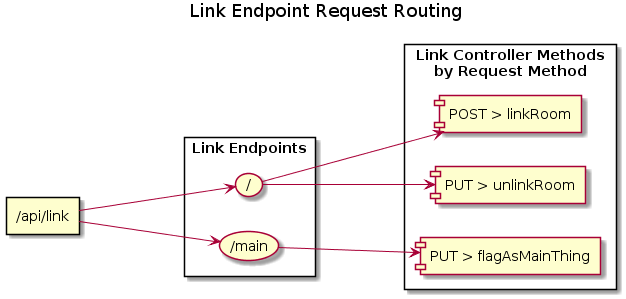
\includegraphics[height=2.5in]{figures/diagrams/back/router-flow/link-endpoints.png}
\caption[link-endpoints]{Link API Schema\footnotemark}
\end{figure}

Para el endpoint \verb|/api/link|, se asocian 3 entradas atendidas por el \verb|link.router.js|:
\begin{enumerate}
\item En la ruta \verb|/api/link/|, las peticiones POST serán atendidas por el método \verb|linkRoom|.
\item En la ruta \verb|/api/link/|, las peticiones PUT serán atendidas por el método \verb|unlinkRoom|.
\item En la ruta \verb|/api/link/main|, las peticiones PUT serán atendidas por el método \verb|flagAsMainThing|.
\end{enumerate}

\begin{figure}[hbt!]
\centering
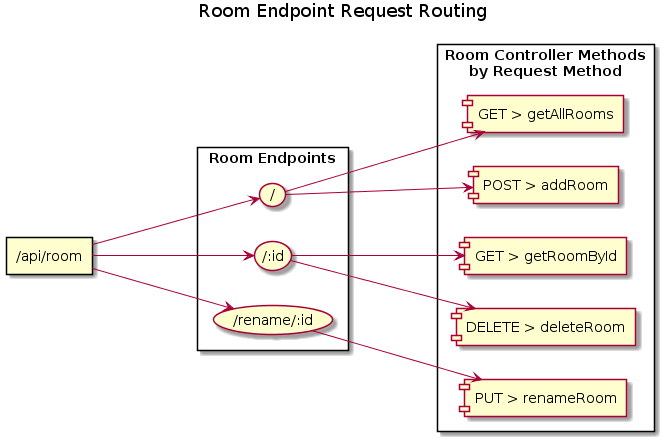
\includegraphics[height=2.5in]{figures/diagrams/back/router-flow/room-endpoints.png}
\caption[room-endpoints]{Room API Schema\footnotemark}
\end{figure}

Para el endpoint \verb|/api/room|, se asocian 5 entradas atendidas por el \verb|room.router.js|:
\begin{enumerate}
\item En la ruta \verb|/api/room/|, las peticiones GET serán atendidas por el método \verb|getAllRooms|.
\item En la ruta \verb|/api/room/|, las peticiones POST serán atendidas por el método \verb|addRoom|.
\item En la ruta \verb|/api/room/:id|, las peticiones GET serán atendidas por el método \verb|getRoomById|.
\item En la ruta \verb|/api/room/:id|, las peticiones DELETE serán atendidas por el método \verb|deleteRoom|.
\item En la ruta \verb|/api/room/rename/:id|, las peticiones PUT serán atendidas por el método \verb|renameRoom|.
\end{enumerate}

\begin{figure}[hbt!]
\centering
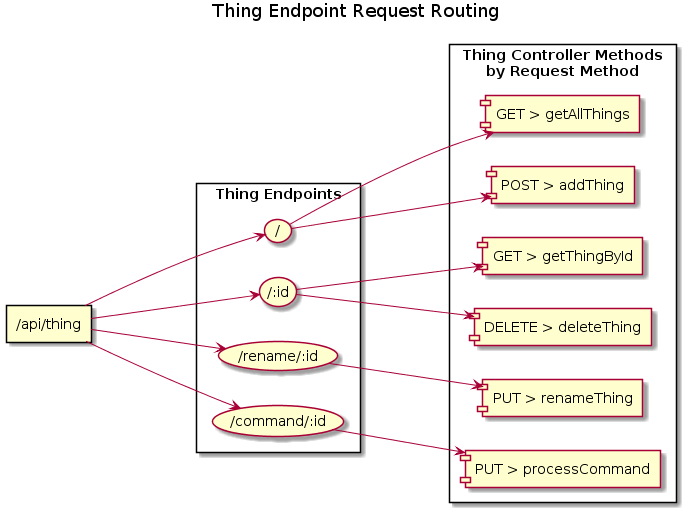
\includegraphics[height=2.5in]{figures/diagrams/back/router-flow/thing-endpoints.png}
\caption[thing-endpoints]{Thing API Schema\footnotemark}
\end{figure}

Para el endpoint \verb|/api/thing|, se asocian 6 entradas atendidas por el \verb|thing.router.js|:
\begin{enumerate}
\item En la ruta \verb|/api/thing/|, las peticiones GET serán atendidas por el método \verb|getAllThings|.
\item En la ruta \verb|/api/thing/|, las peticiones POST serán atendidas por el método \verb|addThing|.
\item En la ruta \verb|/api/thing/:id|, las peticiones GET serán atendidas por el método \verb|getThingById|.
\item En la ruta \verb|/api/thing/:id|, las peticiones DELETE serán atendidas por el método \verb|deleteThing|.
\item En la ruta \verb|/api/thing/rename/:id|, las peticiones PUT serán atendidas por el método \verb|renameThing|.
\item En la ruta \verb|/api/thing/command/:id|, las peticiones PUT serán atendidas por el método \verb|processCommand|.
\end{enumerate}

\begin{figure}[hbt!]
\centering
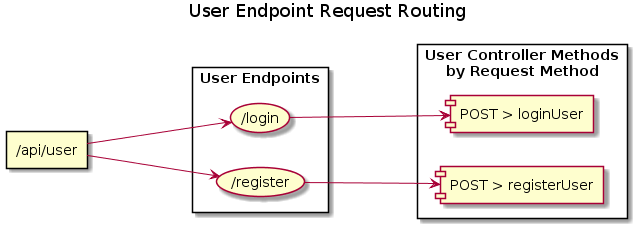
\includegraphics[height=2.5in]{figures/diagrams/back/router-flow/user-endpoints.png}
\caption[user-endpoints]{User API Schema\footnotemark}
\end{figure}

Para el endpoint \verb|/api/user|, se asocian 2 entradas atendidas por el \verb|user.router.js|:
\begin{enumerate}
\item En la ruta \verb|/api/link/login|, las peticiones POST serán atendidas por el método \verb|loginUser|.
\item En la ruta \verb|/api/link/register|, las peticiones POST serán atendidas por el método \verb|registerUser|.
\end{enumerate}

\begin{figure}[hbt!]
\centering
\includegraphics[height=2.5in]{figures/diagrams/back/router-flow/board-endpoints.png}
\caption[board-endpoints]{Board API Schema\footnotemark}
\end{figure}

Para el endpoint \verb|/api/board|, se asocian 2 entradas atendidas por el \verb|board.router.js|:
\begin{enumerate}
\item En la ruta \verb|/api/board/|, las peticiones GET serán atendidas por el método \verb|getAllBoards|.
\item En la ruta \verb|/api/board/detect|, las peticiones GET serán atendidas por el método \verb|getUSBConnectedBoard|.
\end{enumerate}

[HABLAR AQUÍ DE MIDDLEWARES]
[passport.middleware.js]


Toda petición http que no sea encaminada a un método mediante esta metodología será automáticamente rechazada. Esto permite controlar severamente los caminos por los cuales se ejecutará una lógica en base a una petición http, y por ende constituye una medida de seguridad adicional por el principio básico de conocer y controlar todas las posibles entradas al servidor con un flujo único y específico para cada una de ellas, para minimizar brechas de seguridad.

\subsection{Diagramas de clases de los Controllers, Helpers, Models y Providers}
\label{makereference4.6.4}

[HABLAR AQUÍ DE CONTROLLERS]

[core.controller.js
  prepareCoreInstances,
  setupCoreMonitors,
  _launchStoredSubscriptions,
  _releaseDaemons
]

[room.controller.js
initializeRooms
roomDaemon
getAllRooms
getRoomById
addRoom
deleteRoom
renameRoom
]

[thing.controller.js
  initializeThings,
  getThingsByRoom,
  thingDaemon,
  addThing,
  getAllThings,
  getThingById,
  deleteThing,
  renameThing,
  processCommand
]

[link.controller.js
  linkRoom,
  unlinkRoom,
  flagAsMainThing
]

[board.controller.js
  getAllBoards,
  getUSBConnectedBoard
]

[user.controller.js
  getAllBoards,
  getUSBConnectedBoard
]

[HABLAR AQUÍ DE HELPERS]
[thing.helper.js
  translateCommand,
  getThingControllerInstance,
  generateSubscriptionData,
  getModelStructure,
  getDHT11AvgInfo,
  getMQ135AvgInfo
]

[HABLAR AQUÍ DE MODELS]

[Modelo Board, diagrama y corresponde a la collección Boards]
[Modelo Room, diagrama y corresponde a la collección Rooms]
[Modelo Thing, diagrama y corresponde a la collección Things]
[Modelo User, diagrama y corresponde a la collección Users]


[HABLAR AQUÍ DE PROVIDERS]

[mongo.db.js _connect]

[mqtt.service.js
  initializeClient,
  stopClient,
  addSubscription,
  removeSubscription,
  publish
  
  _loadSubscriptions
  _subscribeTopic
  _unsubscribeTopic
  _publishTopic
  _initMessageListener
  _formTopic
  _findSubscriptionIndex
  _processMessage
  ]
  
  [shell.service.js 
  compileAndUploadToBoard
  _execAsync
  ]

  [usb.service.js 
  initListening,
  stopListening,
  getCurrentConnectedUSB,
  ]

\section{Instalación y configuración del nodo principal}
\label{makereference4.7}
 Utilizando los repositorios de distribuciones oficiales de Sistemas operativos de Raspberry Pi, descargamos la versión ``Lite'' de Raspbian. Para establecer una conexión SSH por terminal es necesario crear un fichero con nombre \verb|ssh| en la raiz de la unidad de almacenamiento donde previamente se haya montado la imagen descargada. La distribución de Raspbian originalmente estaba configurada por defecto con la conexión de SSH abierta en el puerto 22, pudiendo accederse con el usuario \verb|pi| y la contraseña \verb|raspberry|. Este dato era ignorado por los usuarios menos experimentados y esto supuso una brecha de seguridad en todos las distribuciones que no fueron configuradas a posteriori por los usuarios según las indicaciones de la propia \href{https://www.raspberrypi.org/documentation/configuration/security.md}{documentación de Raspberry}~\cite{securingyourraspberrypi}. En el primer arranque del SO de la Raspberry se establecerán las configuraciones básicas para las sucesivas conexiones SSH basadas en autenticación con claves privadas.

 De las estrategias disponibles para esta configuración, se crearán las claves en el equipo remoto que se conectará a la Raspberry, entregando mediante la primera conexión SSH con terminal la clave pública y almacenando la clave privada en el equipo remoto, reduciendo así el riesgo de ser expuesta fuera del dominio local del equipo. Para disponer de flexibilidad de conexión independientemente del SO del equipo remoto, la clave privada tendra un formato OpenSSH, fácil de incluir en SO Windows ya sea mediante conversión de la clave a formato PPK o como fichero accesible para aplicaciones de desarrollo, transferencias de ficheros, y/o control de versiones que integran conexiones SSH configurables (GitHub, Filezilla, Eclipse, etc). Los pasos necesarios para establecer conexiones cifradas robustas pueden encontrarse en el Anexo A seccion de implementación del Gateway.

Establecemos la capacidad de la Raspberry Pi 3 para su módulo de comunicación wifi de actuar como punto de acceso en modo NAT~\cite{raspberrypiasaccesspoint}. Se configura una red con acceso vía usuario y contraseña, con WPA2 y gestión de claves WPA-PSK. De esta forma, el nodo será capaz de desplegar una red inalámbrica que permitirá a otros dispositivos incorporarse a la suite domótica.

En orden de subir sketcs a una Arduino desde una Raspeberry Pi, es necesario instalar las paqueterías del compilador sudo apt-get install arduino-mk, tras la instalación, en la ruta /usr/sahre/arduino pueden encontrar binarios y una capeta llamada examples que permiten cargan sketchs inmediatamente para comprobar el correcto funcionamiento del la placa microcontroladora. Para compilar dicho sketcs se necesita hacer referencia al fichero arduino.mk. De los ejemplo podemos verificar rampidamente el correcto funcionamiento de la microcontroladores utilizamos el mas básico de los \gls{sketch}, situado en /usr/share/arduino/examples/01.Basic/Blink/Blink.ino, este ejemplo es muy básico, un loop que enciende y apaga el led integrado en la placa microcontroladora cada 1000 milisegundos. Este , es por defecto el sketch que generelamente los disitntos fabricantes de placas microcontroladoras de con procesador ATmega328P suelen dejar cargado a modo de test. Alterando el valor basico de sleep entre lineas de encendido y apagado a un valor menor como 50 milisegundos se puede comprobar si la comunicación del puerto com, y el compilador suben correctamente el codigo a la placa. Es importante verificar este punto antes de continuar y esta simple prueba cofirma que la configuración actual esta bien.

Para facilitar el proceso de subida de codigo a la placa de arduino, crearemos un Makefile hijo que enlace parametros al compilador.


Ahora bien, tengamos en cuenta que las especificaciones del modulo esp8266 de wifi conectado a Arduino requieren de una alimentación de 3.3V que pueden ser suministrados por la placa microcontroladora, sin embargo, esto nos deja con un problema de intensidad en la alimentación del modulo, ya que el pin de 3.3V disponible en la placa posees un amperaje de 50mA y se requieren de unos 200mA para garantizar una comunicación estable.


mqtt
\url{https://theembeddedlab.com/tutorials/install-mosquitto-on-a-raspberry-pi}
\verb|-h BROKER -t TOPIC|

\verb|mosquittosub -h localhost -t casa/comedor/temperatura|
\verb|mosquittopub -h localhost -t casa/comedor/temperatura -m "Temperatura: 25ºC"|


usando comunicacion cifrada en nodeucm esp8266
https://github.com/esp8266/arduino-esp8266fs-plugin
cifrado tls open source
\url{https://github.com/esp8266/Arduino/blob/master/libraries/ESP8266WiFi/src/WiFiClientSecure.h#L52-L66}